\chapter{Dimensionner et analyser}
Il faudra respecter les contraintes globales portant sur la résolution, la précision (budget des erreurs), délai (budget des temps), immunité aux parasites (liée à la nature des références), en fonction de la structure générale de la chaîne et des propriétés de chacun des composants.
\section{Structure de la chaîne}
\subsection{Récapitulatif des éléments de base}
Les modules qui ont une position fixée dans la chaîne sont:
\begin{itemize}
	\item transducteur + conditionneur (dont pré-ampli) = source
	\item filtre (anti-repliement)
	\item Sample \& Hold (échantillonneur/bloqueur)
	\item CAN
\end{itemize}
\begin{figure}[H] 
	\centering 
	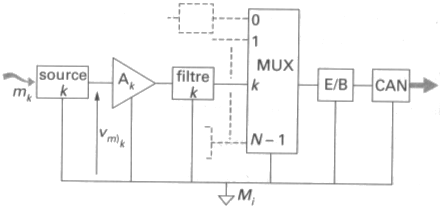
\includegraphics[width=0.8\textwidth,height=10\baselineskip,keepaspectratio]{ch6/image1} 
	\caption{Structure de la chaîne} 
	\label{fig:strucchain}
\end{figure}
Les modules dont la position peut varier sont:
\begin{itemize}
	\item amplificateur, permettant l'ajustement du niveau à celui du CAN. Peut être avant ou après le multiplexeur
	\item multiplexeur (à priori avant le S\&H)
\end{itemize}
\subsection{Options pour l'amplification}
\subsubsection{Un ampli par voie}
Il sera donc avant le multiplexeur, de gain fixe. Il possède une meilleure immunité aux parasites et aux décalages des modules suivants mais coûte plus cher s'il y a beaucoup de voie (N amplis)
\subsubsection{Un ampli unique}
Il sera donc après le multiplexeur, de gain programmable. Ça coûte moins cher s'il y a beaucoup de voie, au détriment d'un délai de réglage du gain et une moins bonne immunité aux parasites et aux décalages des modules suivants.
\subsection{Options pour le moment d'acquisition}
\subsubsection{Acquisition séquentielle}
On mesure N grandeurs à des instants différents. \(T_{ech}\ll\ (f_{ech}\gg)\) délai de variation (cste de temps) des processus. 
\subsubsection{Acquisition simultanée}
On mesure N grandeurs simultanément. \(T_{ech}\approx\) délai des variation des processus. Ça demande 1 S\&H par voie\\
N.B.: la quantification et/ou lecture du résultat restent séquentielles.
\subsection{Parcours des différents cas}
On a donc plusieurs cas que l'on va vite décrire ici
\begin{enumerate}
	\item échantillonnage séquentiel
	\begin{enumerate}
		\item références identiques
		\begin{enumerate}
			\item 1 ampli par voie: ampli asymétrique (gain fixe) et multiplexeur unipolaire (\autoref{fig:strucchain})
			\item 1 ampli unique: ampli asymétrique (gain programmable) et multiplexeur unipolaire (\autoref{fig:seqiu})
		\end{enumerate}
		\item références distinctes
		\begin{enumerate}
			\item 1 ampli par voie: ampli différentiel (gain fixe, ampli d'instrumentation) et multiplexeur unipolaire (\autoref{fig:seqdv})
			\item 1 ampli unique: ampli différentiel (gain programmable) et multiplexeur bipolaire (\autoref{fig:seqdu})
		\end{enumerate}
	\end{enumerate}
	\item échantillonnage simultané (rappel: 1 S\&H par voie)
	\begin{enumerate}
		\item références identiques
		\begin{enumerate}
			\item 1 CAN unique: \(T_{ech}\geq N \) conversion A/N (\autoref{fig:simiu})
			\item 1 CAN par voie: une chaîne complète par voie, plus rapide car \(T_{ech}\geq 1\) conversion A/N (hyp: conversion bcp + lente que lecture) (\autoref{fig:simiv})
		\end{enumerate}
	\end{enumerate}
\end{enumerate}
\begin{figure}[H]
	\centering
	\subfigure[séquentiel, indentiques, ampli unique]{\label{fig:seqiu}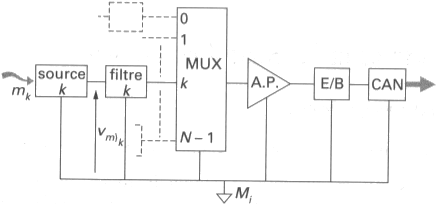
\includegraphics[width=.5\textwidth]{ch6/image2}}
	\subfigure[séquentiel, distinctes, ampli par voie]{\label{fig:seqdv}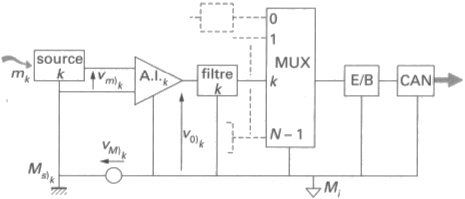
\includegraphics[width=.5\textwidth]{ch6/image3}}%
	\subfigure[séquentiel, disctinctes, ampli unique]{\label{fig:seqdu}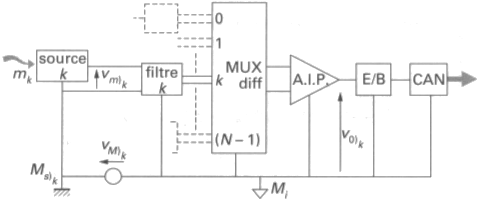
\includegraphics[width=.5\textwidth]{ch6/image4}}
	\subfigure[simultané, indentiques, mux unique]{\label{fig:simiu}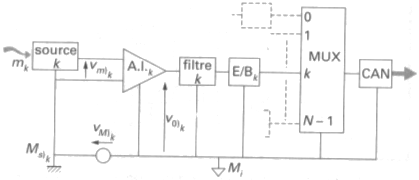
\includegraphics[width=.5\textwidth]{ch6/image5}}%
	\subfigure[simultané, indentiques, mux par voie]{\label{fig:simiv}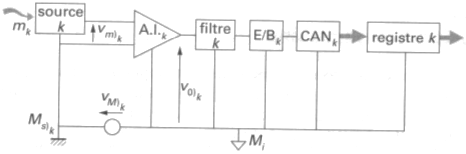
\includegraphics[width=.5\textwidth]{ch6/image6}}
	\caption{Type de structure de chaîne d'acquisition}
\end{figure}
\section{Gain de la chaîne}
\subsection{Récapitulatif des gains}
\begin{itemize}
	\item processus: source du signal délivrant une grandeur physique de valeur 'm'
	\item capteur (transducteur + conditionneur): sensibilité S dans l'hypothèse d'un capteur linéaire (S = cste)
	\item amplificateur: gain \(G_a\), \textbf{à dimensionner}
	\item filtre(s): gain \(G_f\), \textbf{en principe} \(G_f = 1\)
	\item S\&H et mux: gain 1
	\item CAN (quantification): à N bits, de résolution \(q=LSB=V_{FSR}/2^N\).
	\begin{itemize}
		\item valeur d'entrée (analogique) du CAN = \(m.S.G_a.G_f\)
		\item valeur de sortie (numérique) du CAN : \(M=\text{round}(m.S.G_a.G_f/q)\)
	\end{itemize}
\end{itemize}
\subsection{Dimensionnement du gain de l'ampli}
Il faut que la tension d'entrée du CAN couvre tout l'étendue de mesure de celui-ci sinon on perd en SNR et en dynamique.\bigbreak

Critère de dimensionnement de l'ampli: pleine échelle pour \(m_{max}\)
\[\Rightarrow V_{FSR} = m_{max}.S.G_a.G_f\]
\[\Leftrightarrow G_a=\frac{V_{FSR}}{m_{max}.S.G_f}\]
Pour un ampli à gain variable, ce sont souvent des puissances de 2 ou 10 et le gain peut se régler automatiquement.
\section{Résolution de la chaîne}
\subsection{Limite de résolution due au CAN}
Pour rappel, la résolution est la plus petite variation détectable et correspond à 1 LSB = \(q = V_{FSR}/2^N\).\\
À la sortie du conditionneur, on a \(\delta v=q/(G_a.G_f)\) et au niveau du processus \begin{itemize}
	\item[\(\bullet\)] \(\delta m = q/(G_a.G_f.S)\) (hyp: capteur lin.)
	\item[\(\bullet\)] \(\delta m = m_{max}/2^N\) (hyp: gain ampli ok selon précédent critère) \(\Rightarrow\) augmenter N permet une meilleure résolution (CAN seul).
\end{itemize}
\subsection{Dimensionnement du CAN}
La résolution effective du dispositif est limité par:
\begin{itemize}
	\item le bruit de fond sur le signal analogique (\(V_b^2\)) (dû au processus et modules en amont)
	\item le bruit de quantification dû au CAN (\(V_{b_{CAN}}^2=q^2/12\))
\end{itemize}
Les 2 bruits doivent être du même ordre: le bruit de quantification doit être < bruit de fond mais ça sert à rien de descendre nettement sous le bruit de fond \(\Rightarrow\) critère de dimensionnement
\[V_{b_{CAN}}^2\leq V_b^2\Rightarrow \frac{V_{FSR}}{2^N}\leq\sqrt{12V_b^2}\Rightarrow N\geq\num{3.3}\log\!\left(\frac{V_{FSR}}{V_b}\right)-\num{1.8}\]
\section{Dimensionnement temporel}
2 problèmes:
\begin{itemize}
	\item coordination des modules = séquencement correct des opérations (vu grossièrement)
	\item temps nécessaire à chaque acquisition (fréquence d'échantillonnage/ temps de scrutation)	
\end{itemize}
\subsection{Budget des temps}
Faisons une décomposition temporelle de la chaîne standard (un ampli par voie, structure 1.(a).i \autoref{fig:strucchain}). Il y a donc la source + ampli + filtre qui travaille en continu. Soit l'instant "0" la commande de la voie k du mux., on a:
\begin{itemize}
	\item multiplexeur
	\begin{itemize}
		\item \(t_0\): le mux reçoit l'ordre de sélectionner la voie k \(\rightarrow\) + temps d'établissement à \(\varepsilon\) près (\(t_{\varepsilon,mux}\))
	\end{itemize}
	\item échantillonner/bloqueur
	\begin{itemize}
		\item \(t_1\): S\&H reçoit l'ordre d'échantillonner \(\rightarrow\) + temps d'acquisition à (\(\varepsilon\)) près (\(t_{\varepsilon,acq}\))
		\item \(t_2\): S\&H reçoit l'ordre de bloquer \(\rightarrow\) + temps d'établissement à (\(\varepsilon\)) près (\(t_{\varepsilon,S\&H}\))
	\end{itemize}
	\item CAN
	\begin{itemize}
		\item \(t_3\): CAN reçoit l'ordre de conversion \(\rightarrow\) + temps de conversion (\(t_{CAN}\))
	\end{itemize}
	\item ampli à gain programmable éventuel (entre mux et S\&H)
	\begin{itemize}
		\item à partir de l'instant où il reçoit l'ordre de modifier le gain \(\rightarrow\) + temps d'établissement à \(\varepsilon\) près (\(t_{\varepsilon,ampli}\))
	\end{itemize}
\end{itemize}
On définit le temps de scrutation (mux + modules en aval)
\[t_{src,min} = t_{\varepsilon,mux}+t_{\varepsilon,acq}+t_{\varepsilon,S\&H}+t_{CAN}(+t_{\varepsilon,ampli})\]
Ainsi, on a notre limite max de fréquence d'échantillonnage:
\begin{itemize}
	\item fréquence d'échantillonnage max. du système (= celle du CAN)
	\[f_{s_{max,sys}}=1/t_{scr,min}\]
	\item fréquence d'échantillonnage max. par voie (= un tour de MUX)
	\[_{s_{max,voie}}=1/(N.t_{scr,min})\]
	\item échantillonnage correct d'une voie (Shannon/Nyquist)
	\[f_{s_{min,voie}}=2f_{max,signal}\]
\end{itemize}
Donc le fréquence d'échantillonnage réelle du système est
\[2N.f_{max,signal}<f_{s_{sys}}<1/t_{scr,min}\]
\begin{figure}[H] 
	\centering 
	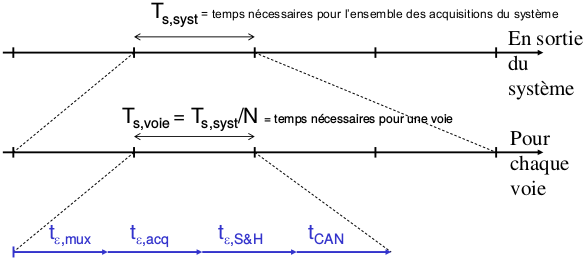
\includegraphics[width=0.6\textwidth,height=10\baselineskip,keepaspectratio]{ch6/image7} 
	\caption{Budget de temps} 
\end{figure}
\begin{figure}[H] 
	\centering 
	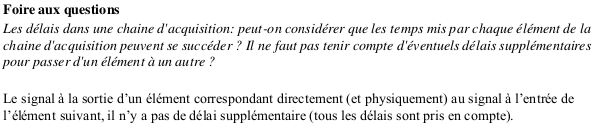
\includegraphics[width=0.8\textwidth,height=10\baselineskip,keepaspectratio]{ch6/image8}  
\end{figure}
\begin{figure}[H] 
	\centering 
	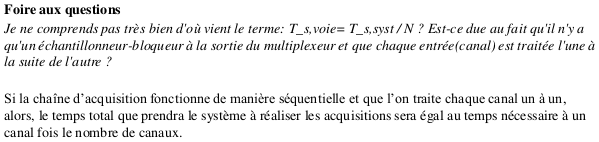
\includegraphics[width=0.8\textwidth,height=10\baselineskip,keepaspectratio]{ch6/image9}  
\end{figure}
\begin{figure}[H] 
	\centering 
	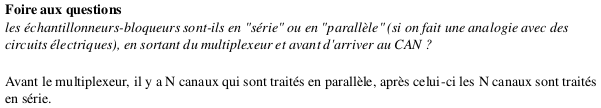
\includegraphics[width=0.8\textwidth,height=10\baselineskip,keepaspectratio]{ch6/image10}  
\end{figure}
\subsection{Réduction du temps de scrutation}
\subsubsection{Multiplexage anticipé}
Pendant que le CAN convertit la sortie du S\&H pour la voie k (qui est invariant tant qu'on ne commute pas le S\&H), le MUX est déjà commuté sur la voie k+1. On gagne le temps d'établissement du MUX car il s'effectue en \(\parallelsum\) avec la conversion. Critère: \(t_{CAN}\geq t_{\varepsilon,mux}\)
\subsubsection{Échantillonnage alterné ("ping-pong")}
On utilise 2 échantillonneur/bloqueurs pour un CAN. S\&H\(_1\) échantillonne la voie 1 (mode échantillonnage) pendant que S\&H\(_2\) est en mode blocage et le CAN en conversion. On parallélise l'échantillonnage et le blocage.
\subsection{Signaux à fréquences hautes distinctes}
C'est au niveau du multiplexeur que ça se passe
\subsubsection{Multiplexeur échelonné}
Constitué de 2 multiplexeurs en cascade, le 1\up {er} étant plus rapide que le 2\up{ème}.
\subsubsection{Multiplexage réparti}
On applique le même signal sur plusieurs voies d'un même multiplexeur (le nombre de voies dépend de la fréquence à atteindre)
\section{Précision de la chaîne}
\subsection{Cas idéal}
Chaque module ajoute un facteur multiplicatif entre son entrée et sa sortie (gain \(G_i\))
\[y_k=G_k.x_k\]
\subsection{Cas réel}
Chaque module introduit une erreur sur sa sortie par rapport au modèle précédent (erreur de gain, décalage, de dérivé, l'influence de la fréquence, etc.)
\[y_k=G_k.x_k\pm \delta y_k\]
À la sortie de la chaîne (valeur numérique), on a
\[N=G_{\text{total}}m\pm\delta N\]
l'erreur de précision relative est donc \(\delta N/N_{max}\). L'erreur du module k est multiplié par tous les gain de tous les modules qui suivent.\\
On peut montre que l'erreur relative globale est la somme des erreurs relatives dues à chacun des modules
\[\varepsilon=\sum_1^n\varepsilon_k\]
On définit aussi

\[\text{erreur maximale ("worst case")}\qquad\text{erreur probable (moy. géo.)}\]
\[\varepsilon_{max}=\sum_1^n|\varepsilon_k|\qquad\qquad\varepsilon_{prob}=\sqrt{\sum_1^n\varepsilon_k^2}\]
\section{Synthèse}
\begin{itemize}
	\item Structure de la chaîne
	\begin{itemize}
		\item 2 extrêmes : tout en commun >< tout en parallèle. En fonction du coût et délai/précision
	\end{itemize}
	\item Ampli
	\begin{itemize}
		\item gain programmable >< gain fixe. En fonction de,la structure de la chaîne
		\item Si pour une voie: dimensionner suivant le niveau max du signal et de la gamme d'entrée du CAN
	\end{itemize}
	\item CAN
	\begin{itemize}
		\item Dimensionner le nombre de bits en fonction de la résolution
		\item critère: bruit de quantification du même ordre de grandeur que bruit \textbf{déjà présent} sur le signal
	\end{itemize}
	\item S\&H
	\begin{itemize}
		\item critère: \(2Nf_{max,signal}<f_{s_{sys}}<1/t_{scr,min}\) pour le cas standard
		\item \(t_{scr,reel}=\sum t_{etabl}\). Dépend des dispositifs utilisés, de la structure plus ou moins \(\parallelsum\) et de la précision voulue
		\item \danger\ temps d'ouverture du S\&H pour signaux à variation rapide
	\end{itemize}
\end{itemize}
Il y a un exo à partir du slide 39.